\documentclass[a4paper, 12pt]{article} % Font size (can be 10pt, 11pt or 12pt) and paper size (remove a4paper for US letter paper)
\usepackage{amsmath,amsfonts,bm}
\usepackage{hyperref,verbatim}
\usepackage{amsthm,epigraph} 
\usepackage{amssymb}
\usepackage{framed,mdframed}
\usepackage{graphicx,color} 
\usepackage{mathrsfs,xcolor} 
\usepackage[all]{xy}
\usepackage{fancybox} 
% \usepackage{xeCJK}
\usepackage{CJKutf8}
\newtheorem*{adtheorem}{定理}
% \setCJKmainfont[BoldFont=FZYaoTi,ItalicFont=FZYaoTi]{FZYaoTi}
\definecolor{shadecolor}{rgb}{1.0,0.9,0.9} %背景色为浅红色
\newenvironment{theorem}
{\bigskip\begin{mdframed}[backgroundcolor=gray!40,rightline=false,leftline=false,topline=false,bottomline=false]\begin{adtheorem}}
    {\end{adtheorem}\end{mdframed}\bigskip}
\newtheorem*{bdtheorem}{定义}
\newenvironment{definition}
{\bigskip\begin{mdframed}[backgroundcolor=gray!40,rightline=false,leftline=false,topline=false,bottomline=false]\begin{bdtheorem}}
    {\end{bdtheorem}\end{mdframed}\bigskip}
\newtheorem*{cdtheorem}{习题}
\newenvironment{exercise}
{\bigskip\begin{mdframed}[backgroundcolor=gray!40,rightline=false,leftline=false,topline=false,bottomline=false]\begin{cdtheorem}}
    {\end{cdtheorem}\end{mdframed}\bigskip}
\newtheorem*{ddtheorem}{注}
\newenvironment{remark}
{\bigskip\begin{mdframed}[backgroundcolor=gray!40,rightline=false,leftline=false,topline=false,bottomline=false]\begin{ddtheorem}}
    {\end{ddtheorem}\end{mdframed}\bigskip}
\newtheorem*{edtheorem}{引理}
\newenvironment{lemma}
{\bigskip\begin{mdframed}[backgroundcolor=gray!40,rightline=false,leftline=false,topline=false,bottomline=false]\begin{edtheorem}}
    {\end{edtheorem}\end{mdframed}\bigskip}
\newtheorem*{pdtheorem}{例}
\newenvironment{example}
{\bigskip\begin{mdframed}[backgroundcolor=gray!40,rightline=false,leftline=false,topline=false,bottomline=false]\begin{pdtheorem}}
    {\end{pdtheorem}\end{mdframed}\bigskip}

\usepackage[protrusion=true,expansion=true]{microtype} % Better typography
\usepackage{wrapfig} % Allows in-line images
\usepackage{mathpazo} % Use the Palatino font
\usepackage[T1]{fontenc} % Required for accented characters
\linespread{1.05} % Change line spacing here, Palatino benefits from a slight increase by default

\makeatletter
\renewcommand\@biblabel[1]{\textbf{#1.}} % Change the square brackets for each bibliography item from '[1]' to '1.'
\renewcommand{\@listI}{\itemsep=0pt} % Reduce the space between items in the itemize and enumerate environments and the bibliography

\renewcommand{\maketitle}{ % Customize the title - do not edit title
  % and author name here, see the TITLE block
  % below
  \renewcommand\refname{参考文献}
  \newcommand{\D}{\displaystyle}\newcommand{\ri}{\Rightarrow}
  \newcommand{\ds}{\displaystyle} \renewcommand{\ni}{\noindent}
  \newcommand{\pa}{\partial} \newcommand{\Om}{\Omega}
  \newcommand{\om}{\omega} \newcommand{\sik}{\sum_{i=1}^k}
  \newcommand{\vov}{\Vert\omega\Vert} \newcommand{\Umy}{U_{\mu_i,y^i}}
  \newcommand{\lamns}{\lambda_n^{^{\scriptstyle\sigma}}}
  \newcommand{\chiomn}{\chi_{_{\Omega_n}}}
  \newcommand{\ullim}{\underline{\lim}} \newcommand{\bsy}{\boldsymbol}
  \newcommand{\mvb}{\mathversion{bold}} \newcommand{\la}{\lambda}
  \newcommand{\La}{\Lambda} \newcommand{\va}{\varepsilon}
  \newcommand{\be}{\beta} \newcommand{\al}{\alpha}
  \newcommand{\dis}{\displaystyle} \newcommand{\R}{{\mathbb R}}
  \newcommand{\N}{{\mathbb N}} \newcommand{\cF}{{\mathcal F}}
  \newcommand{\gB}{{\mathfrak B}} \newcommand{\eps}{\epsilon}
  \begin{flushright} % Right align
    {\LARGE\@title} % Increase the font size of the title
    
    \vspace{50pt} % Some vertical space between the title and author name
    
    {\large\@author} % Author name
    \\\@date % Date
    
    \vspace{40pt} % Some vertical space between the author block and abstract
  \end{flushright}
}

% ----------------------------------------------------------------------------------------
%	TITLE
% ----------------------------------------------------------------------------------------
\begin{document}
\begin{CJK}{UTF8}{gkai}
  \title{\textbf{例13.2}} 
  % \setlength\epigraphwidth{0.7\linewidth}
  \author{\small{叶卢庆}\\{\small{杭州师范大学理学院,学号:1002011005}}\\{\small{Email:h5411167@gmail.com}}} % Institution
  \renewcommand{\today}{\number\year. \number\month. \number\day}
  \date{\today} % Date
  
  % ----------------------------------------------------------------------------------------
  
  
  \maketitle % Print the title section
  
  % ----------------------------------------------------------------------------------------
  %	ABSTRACT AND KEYWORDS
  % ----------------------------------------------------------------------------------------
  
  % \renewcommand{\abstractname}{摘要} % Uncomment to change the name of the abstract to something else
  
  % \begin{abstract}
  
  % \end{abstract}
  
  % \hspace*{3,6mm}\textit{关键词:}  % Keywords
  
  % \vspace{30pt} % Some vertical space between the abstract and first section
  
  % ----------------------------------------------------------------------------------------
  %	ESSAY BODY
  % ----------------------------------------------------------------------------------------
  \begin{example}[13.2]
如图显示的是从原点到 $(1,1,1)$ 的另一路径.将 $f(x,y,z)=x-3y^2+z$ 在
$C_1\bigcup C_2$ 上积分.\\
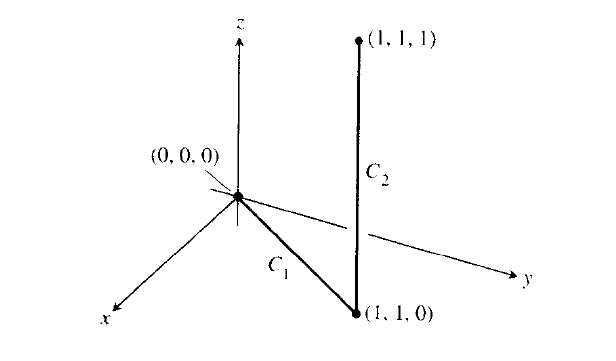
\includegraphics[width=0.8\textwidth]{/home/luqing/Thomas-calculus-10th-edition/example13-2.png}    
  \end{example}
  \begin{proof}[解]
我们悲哀地发现,$C_1\bigcup C_2$ 并不是连续可微的曲线.然而幸运的是,去掉
$(1,1,0)$ 附近的那些导致不连续可微的点,不会影响积分.我们将 $C_1$ 写成
参数方程的形式:
$$
\begin{cases}
  x=t,\\
y=t,\\
z=0
\end{cases}
$$
其中 $0\leq t\leq 1$.因此
$$
\int_0^1(t-3t^2)\sqrt{2}dt=\frac{-\sqrt{2}}{2}.
$$
将 $C_2$ 写成参数方程的形式:
$$
\begin{cases}
  x=1,\\
y=1,\\
z=t,\\
\end{cases}
$$
其中 $0\leq t\leq 1$.因此
$$
\int_0^1(t-2)dt=\frac{-3}{2}.
$$
因此结果为
$$
\frac{-\sqrt{2}-3}{2}.
$$

  \end{proof}
  % ----------------------------------------------------------------------------------------
  %	BIBLIOGRAPHY
  % ----------------------------------------------------------------------------------------
  
  \bibliographystyle{unsrt}
  
  \bibliography{sample}
  
  % ----------------------------------------------------------------------------------------
\end{CJK}
\end{document}